%%% ---------------
%%% PREAMBLE
%%% ---------------
\documentclass[french,11pt,a4paper]{article}

% Define geometry (without using the geometry package)
\usepackage{geometry}
\geometry{landscape, twocolumn, textwidth=27.5cm, textheight=19.5cm, columnsep=15mm}

%\frenchspacing						% better looking spacing

% Call packages we'll need
\usepackage{graphicx}				% images
\usepackage{amssymb,amsmath}		% math
\usepackage{multicol}				% three-column layout
\usepackage{multirow}
\usepackage{url}					% clickable links
\usepackage{marvosym}				% symbols
\usepackage{wrapfig}				% wrapping text around figures
\usepackage{fontspec}			% font encoding
\usepackage{xunicode}
\usepackage{ragged2e}
\usepackage{titlesec}
\usepackage{framed}
%\usepackage[default]{raleway}
\usepackage{tocvsec2}
% Customize (header and) footer
\usepackage{fancyhdr}
\usepackage{enumitem}
\usepackage{fontawesome}
\usepackage{lipsum}
\usepackage{babel}
%\pagestyle{fancy}
\pagestyle{empty}
\setmainfont{Carlito}

%\titlespacing\section{0pt}{0pt plus 4pt minus 2pt}{0pt plus 2pt minus 2pt}
%\titlespacing\subsection{0pt}{12pt plus 4pt minus 2pt}{0pt plus 2pt minus 2pt}
%\titlespacing\subsubsection{0pt}{12pt plus 4pt minus 2pt}{0pt plus 2pt minus 2pt}

%\newfontfamily\headingfont[]{Arial}
%\titleformat*{\section}{\Large\bfseries\sffamily}
%\titleformat*{\section}{\Large\headingfont}

%\renewcommand{\headrulewidth}{0.0pt}	% no bar on top of page
%\renewcommand{\footrulewidth}{0.4pt}	% bar on bottom of page

%%% ---------------
%%% DEFINITIONS
%%% ---------------

% Define separators
\newcommand{\HorRule}[1]{\noindent\rule{\linewidth}{#1}} % Creating a horizontal rule
\newcommand{\SepRule}{\noindent							 % Creating a separator
						\begin{center}
							\rule{250pt}{1pt}
						\end{center}
						}						

% Define Title en News input
\newcommand{\JournalName}[1]{%
		\begin{center}	
			%\Huge \usefont{T1}{augie}{m}{n}
            \Large \usefont{T1}{augie}{m}{n}
			#1%
		\end{center}	
		\par \normalsize \normalfont}
		
\newcommand{\JournalIssue}[1]{%
		\hfill \textsc{\mydate \today, No #1}
		\par \normalsize \normalfont}
\newcommand*{\chants}{../chants}
\newcommand*{\messe}{../messe_bienveillance}
\newcommand*{\pu}{../pu}
\newcommand*{\psaumes}{../psaumes}
\newcommand*{\footer}{..}

\newcommand{\NewsItem}[1]{%
\vspace{3pt}
\underline{\textbf{#1}}
	%	%\usefont{T1}{augie}{m}{n} 	
	%	\large \textbf{#1} %\vspace{3pt}
   %     %\Large #1 \vspace{4pt}
	%	%\par 
   %     \normalsize \normalfont
		  }
		
\newcommand{\NewsAuthor}[1]{%
			\hfill by \textsc{#1} \vspace{4pt}
			\par \normalfont}		

\graphicspath{{../images/}}

%pas de numérotation des sections
\setsecnumdepth{none}
\setlength{\parindent}{0pt}
%%% ---------------
%%% BEGIN DOCUMENT
%%% ---------------
\begin{document}

\NewsItem{CHANT D'ENTRÉE}
	\textbf{Il n’y a pas de petites joies}

R.  Chrétiens réveillez-vous, veilleurs réjouissez-vous,
l’aurore s’est levée, le Fils a triomphé ! Oh non ne vous laissez pas, Oh non ne vous laissez pas voler votre joie, voler votre joie !

1. Depuis que Jésus Christ a pris notre chair, oh non il n’y a pas de petites joies. Depuis que les bergers virent le doux mystère, oh non il n’y a pas de petites joies.

6.
Depuis que Jésus Christ a vaincu la mort, oh non il n’y a pas de petites joies.
depuis que par le feu, l’Esprit nous rend forts oh non il n’y a pas de petites joies.


\NewsItem{PRÉPARATION PÉNITENTIELLE} \\
	Seigneur, prends pitié. Seigneur prends pitié, Seigneur, prends pitié\\
Ô Christ, prends pitié. ô Christ prends pitié, o Christ, prends pitié.\\
Seigneur, prends pitié. Seigneur, prends pitié Seigneur, prends pitié


\NewsItem{GLORIA}
	\begin{itemize}
\item[R/] 
Gloire à Dieu, au plus haut des cieux, et paix sur la terre, aux hommes qu'il aime. (bis)
\item[1.]
Nous te louons, nous te bénissons, nous t’adorons, nous te glorifions, nous   
      te rendons grâce pour ton immense gloire. Seigneur Dieu, Roi du ciel, Dieu 
      le Père tout puissant. R/
\item[2.]
Jésus-Christ, Seigneur Fils unique, Agneau de Dieu, le Fils du Père, toi qui 
      enlèves le péché du monde, reçois nos prières. Toi qui es assis à la droite  
      du Père, prends pitié de nous. R/
\item[3.]
Car toi seul es saint, toi seul es Seigneur, toi seul es le Très Haut : 
      Jésus-Christ, avec le Saint Esprit, dans la gloire de Dieu le Père. R/
\end{itemize}




% -----
\NewsItem{1\iere{} LECTURE} Ac 2, 1-11
% -----

\NewsItem{PSAUME}
Ps 103 (104), 1ab.24ac, 29bc-30, 31.34

\textbf{ Ô Seigneur, envoie ton Esprit qui renouvelle la face de la terre !}

Bénis le Seigneur, ô mon âme ;
Seigneur mon Dieu, tu es si grand !
Quelle profusion dans tes œuvres, Seigneur !
la terre s’emplit de tes biens.

Tu reprends leur souffle, ils expirent
et retournent à leur poussière.
Tu envoies ton souffle : ils sont créés ;
tu renouvelles la face de la terre.

Gloire au Seigneur à tout jamais !
Que Dieu se réjouisse en ses œuvres !
Que mon poème lui soit agréable ;
moi, je me réjouis dans le Seigneur.


% -----
\NewsItem{2\ieme{} LECTURE} Rm 8, 8-17

\NewsItem{ACCLAMATION}
Alleluia \emph{messe du Peuple de Dieu}


\NewsItem{ÉVANGILE} Jn 14, 15-16.23b-26 

\NewsItem{HOMÉLIE}

\NewsItem{PROFESSION DE FOI}

%\newpage

\NewsItem{PRIÈRES UNIVERSELLES} 
Pour les hommes et pour les femmes, pour les enfants de la terre, ton Église qui t’acclame vient te confier sa prière 


\NewsItem{OFFERTOIRE}

\NewsItem{PRIÈRES SUR LES OFFRANDES}
\textit{Nous nous levons et nous répondons : }
Que le Seigneur reçoive de vos mains ce sacrifice à la louange et à la gloire 
de Son nom, pour notre bien et celui de toute l’Église.

\NewsItem{SANCTUS}
Le Seigneur est Saint ! Le Seigneur est Saint ! Le Seigneur est Saint !
Le Seigneur est notre Dieu, Le Seigneur est notre Père. Il règne dans les cieux, qu’Il règne sur la terre.


\NewsItem{ANAMNÈSE}
Christ est venu, Christ est né, Christ a souffert, Christ est mort, 
Christ est ressuscité, Christ est vivant,
Christ reviendra, Christ est là,
Christ reviendra, Christ est là.


\NewsItem{NOTRE PÈRE}

\NewsItem{AGNUS} \\
Agneau de Dieu Qui enlèves le péché du monde, Prends pitié de nous !  Prends pitié de nous ! (bis) \\
Agneau de Dieu Qui enlèves le péché du monde, Donne-nous la paix !  Donne-nous la paix !


\NewsItem{COMMUNION}
Voici le Corps et le Sang du Seigneur

\textbf{Voici le Corps et le Sang du Seigneur, la coupe du salut et le pain de la vie. Dieu immortel se donne en nourriture pour que nous ayons la vie éternelle}

1. Au moment de passer vers le Père le Seigneur prit du pain et du vin,\\
pour que soit accompli le mystère qui apaise à jamais notre faim.

2. Dieu se livre lui-même en partage, par amour pour son peuple affamé.\\
Il nous comble de son héritage afin que nous soyons rassasiés.

3. C'est la foi qui nous fait reconnaître, dans ce pain et ce vin consacrés,\\
la présence de Dieu notre maître le Seigneur Jésus ressuscité.

%4. Que nos langues sans cesse proclament, la merveille que Dieu fait pour nous.\\
%Aujourd'hui il allume une flamme,  afin que nous l'aimions jusqu'au bout.


\NewsItem{CHANT D'ENVOI}
\textbf{IL EST TEMPS DE QUITTER}

R. Il est temps de quitter vos tombeaux,
De sortir du sommeil de la nuit,
D’aller vers la lumière acclamer
Le Dieu trois fois Saint ! (bis)

1. Vainqueur de la nuit, Christ ressuscité,
Tu dévoiles la face du Père.
Tu es la lumière, tu es notre joie.
Sois béni, ô Dieu qui nous libères !

3. Tu donnes l’Esprit, Christ ressuscité, 
Tu déverses les fleuves d’eaux vives.
Fils aimé du Père tu nous as sauvés.
Gloire à toi, pour ta miséricorde !


\newpage


\NewsItem{Intentions de messe}
\begin{itemize}
\item[\Cross]
Roland et Liliane ALBUGUES
\end{itemize}

\NewsItem{Informations paroissiales}

\begin{tabular} {lcp{9cm}}
\multicolumn{3}{c}{\textbf{Saint Jean-Baptiste} } \\ \hline
\textbf{Lundi}    & \textbf{09 juin}  & \emph{Bienheureuse Vierge Marie, Mère de l'Église} \textbf{Messe~09h00} \\ \hline
Mardi    & 10 juin  & Vêpres 18h15. Messe 18h30 \\ \hline
Jeudi    & 12 juin  & 
Exposition du Saint Sacrement à 16h00. Adoration. Salut au Saint Sacrement à 18h15. Messe à 18h30 
 \\ \hline
Vendredi & 13 juin  & Laudes 08h45. Messe 09h00 \\ \hline
Samedi   & 14 juin  & Messe anticipée 18h00 \\ \hline
Dimanche  & 15 juin  & \emph{Sainte Trinité} Messe 11h00 \\ \hline
\multicolumn{3}{c}{\textbf{Sainte Croix} } \\ \hline
Mercredi & 11 juin  & Messe 09h00. \newline \Cross{} \textbf{Enterrement}  14h30 Marie-Claire Noël \\ \hline
Dimanche  & 15 juin  & \emph{Sainte Trinité} Messe 09h30 \\ \hline
%\multicolumn{3}{c}{\textbf{Résidence Landsberg (3 rue Jean Monnet)} } \\ \hline
%Mercredi & 04 juin : & Messe 10h45 \\ \hline
\end{tabular}

\begin{framed}
\begin{tabular} {lcp{8cm}}
\multicolumn{3}{c}{\textbf{Saint Jean-Baptiste} } \\
Dimanche & 15 juin  & 17h00 Concert \og Haut en couleurs \fg avec l'ensemble vocal \textbf{Diapason}. Prix libre. \\
Dimanche & 22 juin  & \emph{Le Saint Sacrement du corps et du sang du Christ}
\mbox{\textbf{Procession}} 09h30 \textbf{Messe} 10h00 (pas de messe à Sainte Croix)\\ \hline
\multicolumn{3}{c}{\textbf{Foyer Oberlin} } \\
Vendredi & 13 juin  & 20h00 - 21h00 \textbf{Nuit des veilleurs}. Venez prier avec l'ACAT pour les victimes des persécutions.
\end{tabular}
\end{framed}


\NewsItem{Répétitions des chorales}
\begin{description}
\item[Chorales paroissiales] : vendredi 20h15 à Sainte Croix
\end{description}

\begin{framed}
\textbf{Presbytère St Jean-Baptiste}
%2 rue de l'école 67380 Lingolsheim 03 88 78 16 45 \\
2 rue de l'école 67380 Lingolsheim \phonenumber[country=FR]{0388781645} \\
\textbf{Permanence} Lun. au Jeu. : 09h30-12h00 et 15h-18h. Ven. 16h-18h00. Sam. 09h30-12h00. \\
\textbf{Courriels} \texttt{nddessables@hotmail.com}, \texttt{danielette67380@gmail.com}

%\textbf{Caritas} Vestiaire ouvert le mardi de 14h à 16h

\texttt{https://stjeanbaptistelingo.fr} \hfill \faFacebook Catho Lingo \hfill \faInstagram @catho\_lingo
\end{framed}



\newpage

\JournalName{Communauté de Paroisses de Lingolsheim \\
\normalsize \textit{Notre Dame des Sables}
%\\ \large \'{E}glise Saint Jean-Baptiste
\\  \normalsize \textit{PENTECÔTE}
\\ \large Samedi 07 juin  2025}
%\noindent\HorRule{3pt} \\[-0.75\baselineskip]
%\HorRule{1pt}
% -----

% Front article
% -----
%\vspace{0.5cm}
%	\SepRule
%\vspace{0.5cm}

%\begin{center}
\begin{minipage}[h]{1.0\linewidth}
 \begin{center}
 \textbf{
 %\dots
\og 
Rentrée Pastorale 2025-2026
 \fg{}
 %\dots
 }
 \end{center}

%\begin{wrapfigure}{l}{1.3cm}
%\vspace{-0.4cm}
%	\includegraphics[scale=1.0]{../images/lazarre}
%\end{wrapfigure}
Une nouvelle rentrée pastorale qui nous réjouit tous. En effet, après un temps de répit, il nous revient de mettre en marche la machine de nos activités pastorales.

Au début de cette nouvelle année pastorale, je souhaite vous redire toute ma joie de vous retrouver pour continuer la mission qui m’est assignée dans notre communauté de paroisses. Et comme chaque année, nous mettrons l’accent en premier lieu sur la vie catéchétique des enfants et des adolescences, l’animation liturgique, la création d’une troisième chorale, la visite aux malades et dans notre maison de retraite ( \emph{Résidence du Parc}), l’accueil et l’accompagnement en vue de baptêmes,  du catéchuménat des adultes, des mariages, l’encadrement  des servants d’autel, l’entretien de notre église pour la rendre  accueillante, avec ces innombrables petits gestes de service qui jalonnent l’existence ; tout cela nous aidera à vivre une véritable dimension ecclésiale.

Je voudrais vous remercier de tout cœur, vous tous qui êtes des membres vivants et actifs de la communauté paroissiale que nous formons, véritable artisans de l’évangélisation ordinaire. Mon souhait pour la vie de notre communauté de paroisses est que nous arrivions toujours plus à nous ouvrir et à nous connaître les uns les autres, à nous apprécier dans ce que nous sommes et vivons.

L’année dernière, avec toutes les entités de nos deux paroisses, nous avons eu différentes propositions, activités et invitations qui ont favorisées l’\textbf{Unité et l’ouverture} qui constituaient notre thème pastoral. Ne manquons pas cette année ces moments simples et conviviaux qui permettent de tisser des liens gratuits, profonds et tout simplement chrétiens.

\begin{wrapfigure}{l}{1.2cm}
\vspace{-0.4cm}
	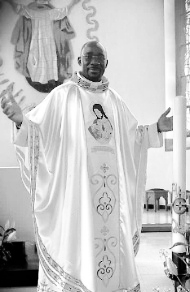
\includegraphics[scale=1.20]{../images/standing_daniel}
\end{wrapfigure}
Cette année nous porterons ensemble cette rentrée dans le cœur de chacun avec nos \textbf{jeunes pro}. Chacun à son rythme, selon ses possibilités et ses réalités mais avec un seul et même objectif : l’accomplissement de nos activités communautaires. Présentons également notre rentrée paroissiale au Christ. Et continuons notre chemin pour la mise en œuvre de notre projet paroissial autour de ce principal thème : \textbf{\og Avec notre jeunesse bâtissons une communauté plus dynamique, rayonnante et missionnaire\fg{}.}

	Que cette rentrée pastorale nous aide à prendre des résolutions nécessairement pour plonger à frais nouveaux dans la parole et être des disciples crédibles de l’évangile.


\begin{flushright}
Bonne rentrée pastorale à toutes et à tous !
\textit{Père  Daniel  ETTÉ}
\end{flushright}


%\lipsum[1-3]
\end{minipage}
%\end{center}
% -----
\end{document} 
